\section{Câu 1}
    \hspace*{0.6cm}\textbf{Tính toán chọn vùng làm việc cho camera so sánh với thực tế và tính toán}
    \subsection{Xác định các thông số sử dụng cho tính toán}
        \subsubsection{Lựa chọn camera}
            \hspace*{0.6cm}Nhóm sử dụng camera Basler a2A1920-51gcBAS với các thông số cần sử dụng:
            \begin{itemize}
                \item Resolution: 1920x1200 pixels
                \item Sensor size: 6.6mm x 4.1mm
                \item Focal Length: 8mm
            \end{itemize}
            \begin{figure}[H]
                \centering
                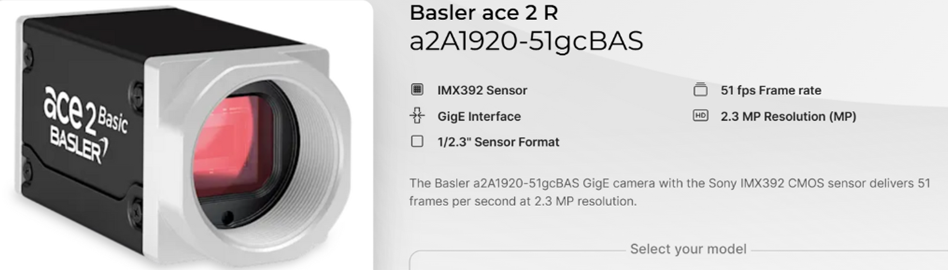
\includegraphics[width=1\textwidth]{pictures/section1/s1_p01.png}
                \caption{Thông số camera Basler a2A1920-51gcBAS}
                \label{fig:camera_basler}
            \end{figure}
            \begin{figure}[H]
                \centering
                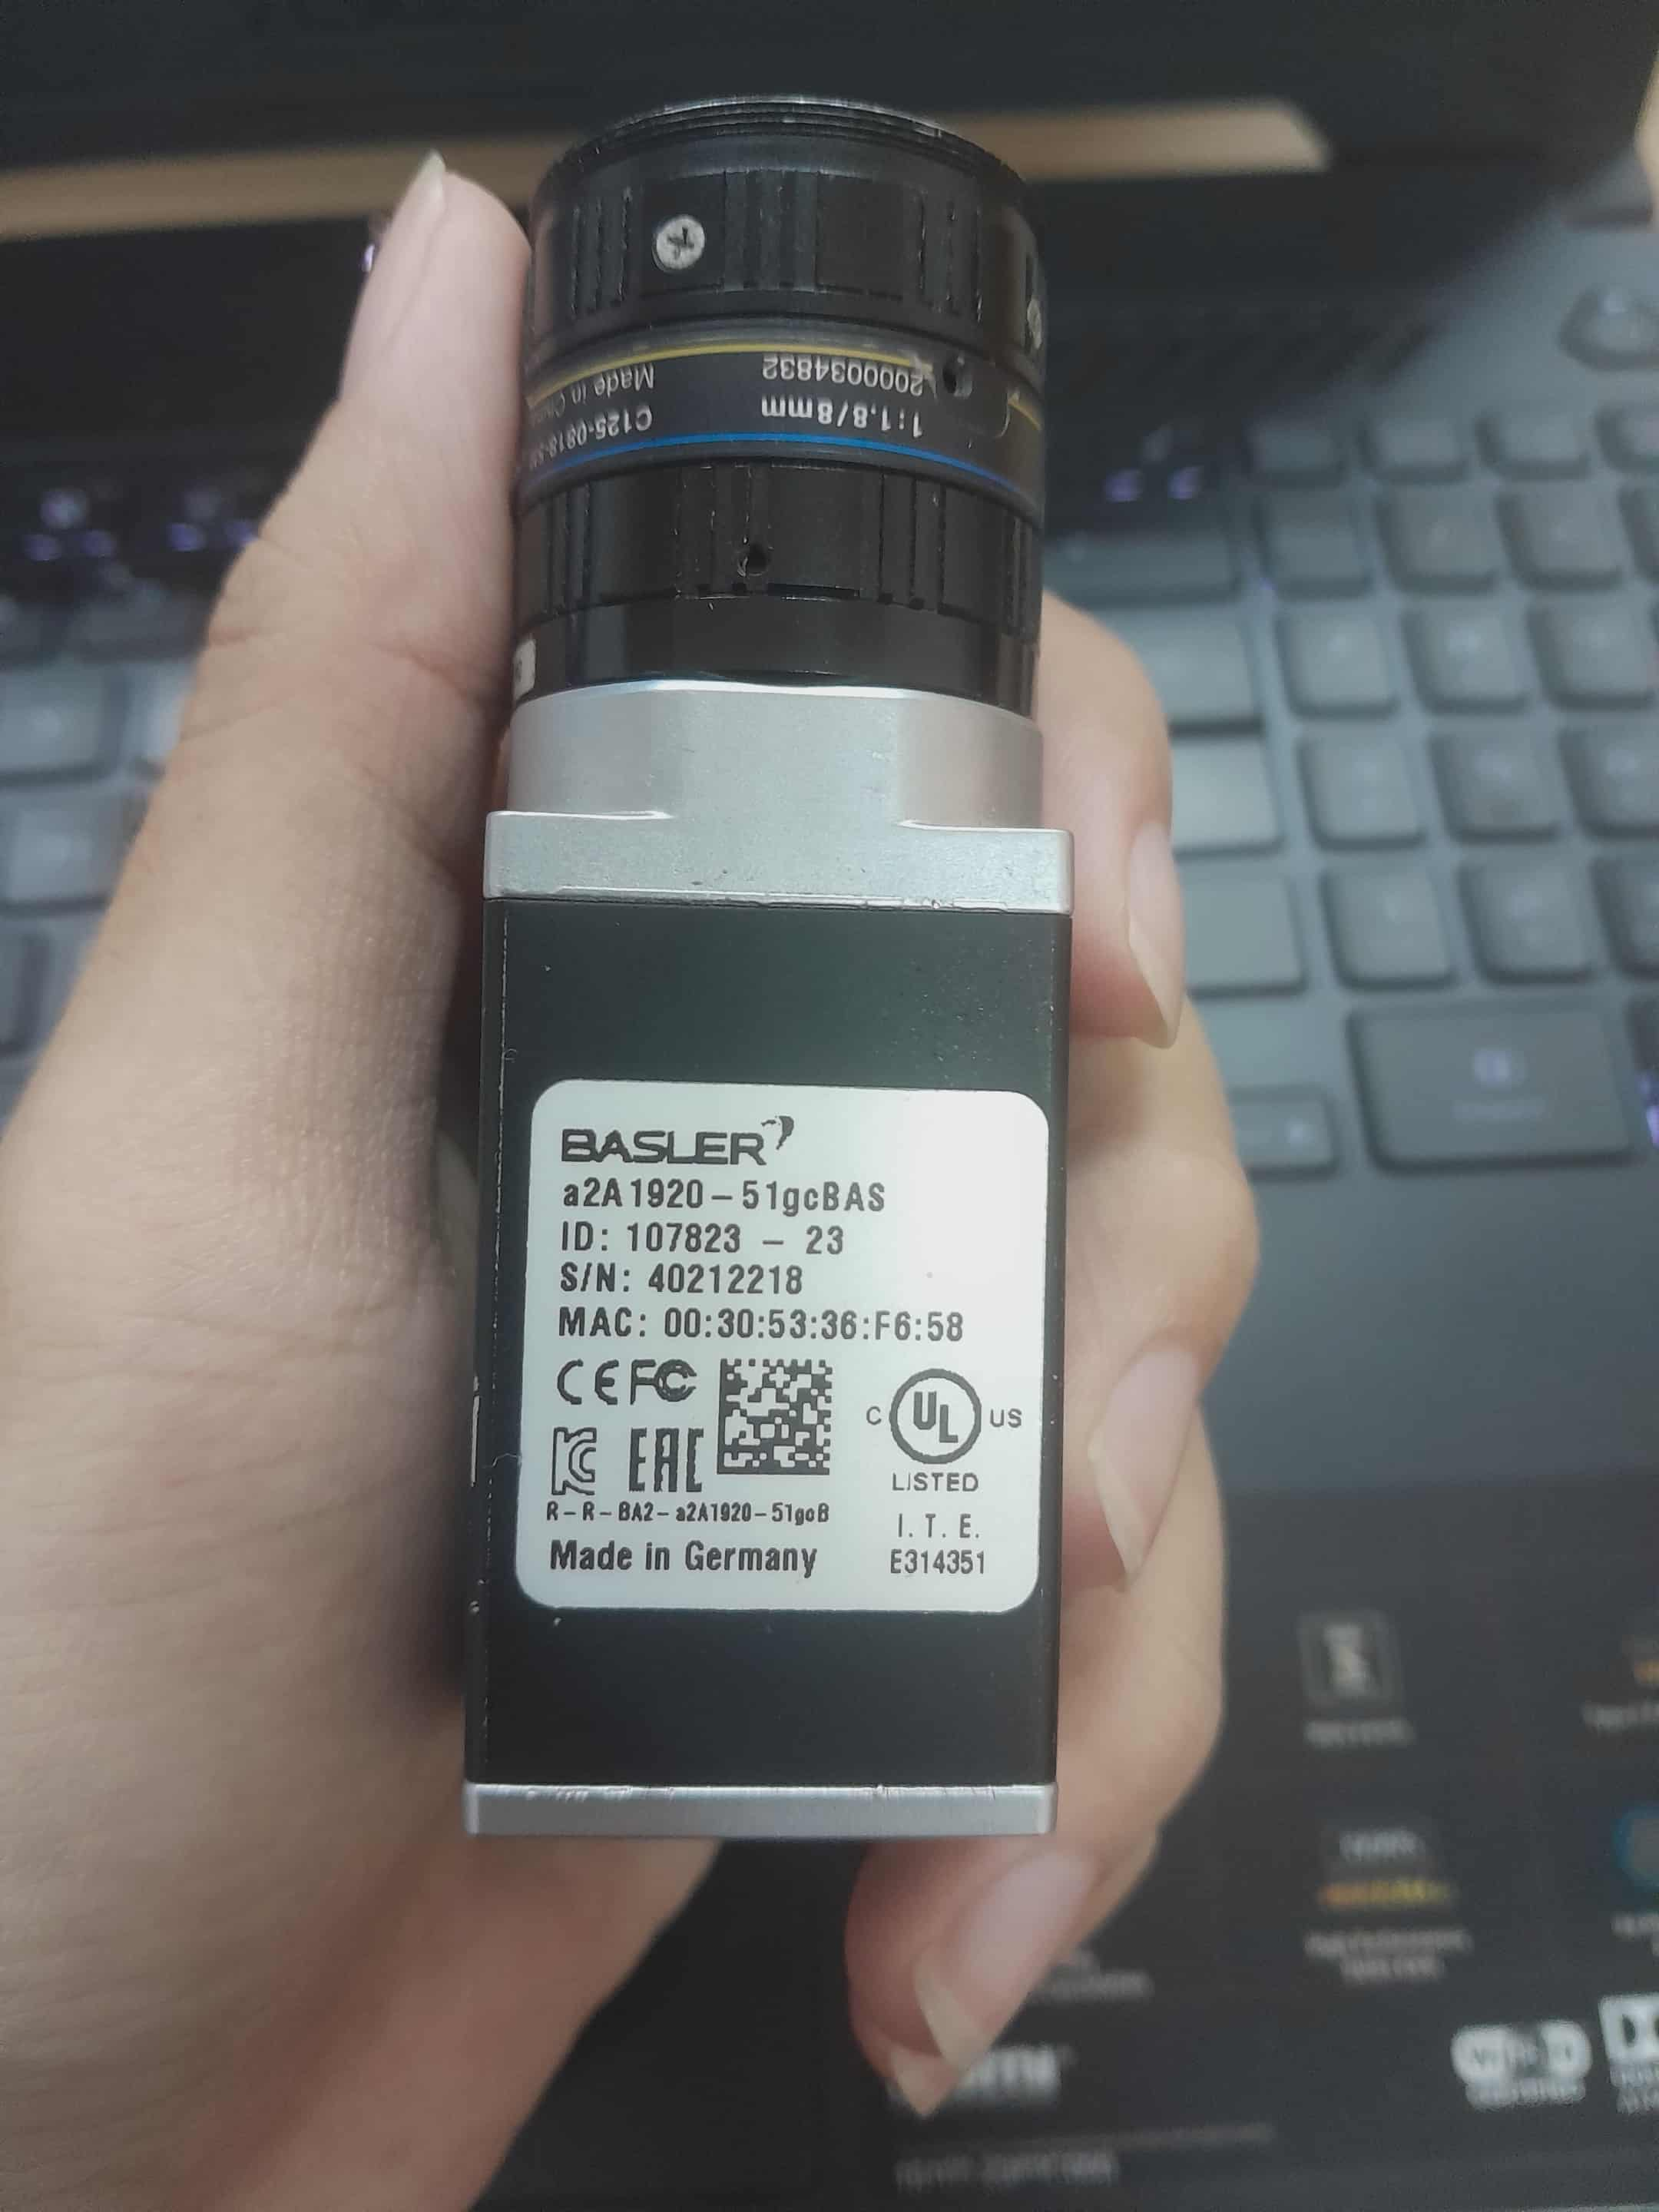
\includegraphics[width=0.4\textwidth]{pictures/section1/s1_p02.png}
                \caption{Hình ảnh thực tế của camera Basler a2A1920-51gcBAS}
                \label{fig:camera_basler}
            \end{figure}

        \subsubsection{Lựa chọn Working Distance}  
            \hspace*{0.6cm}Nhóm tiến hành chọn trước Working Distance: 445 mm
            \begin{figure}[H]
                \centering
                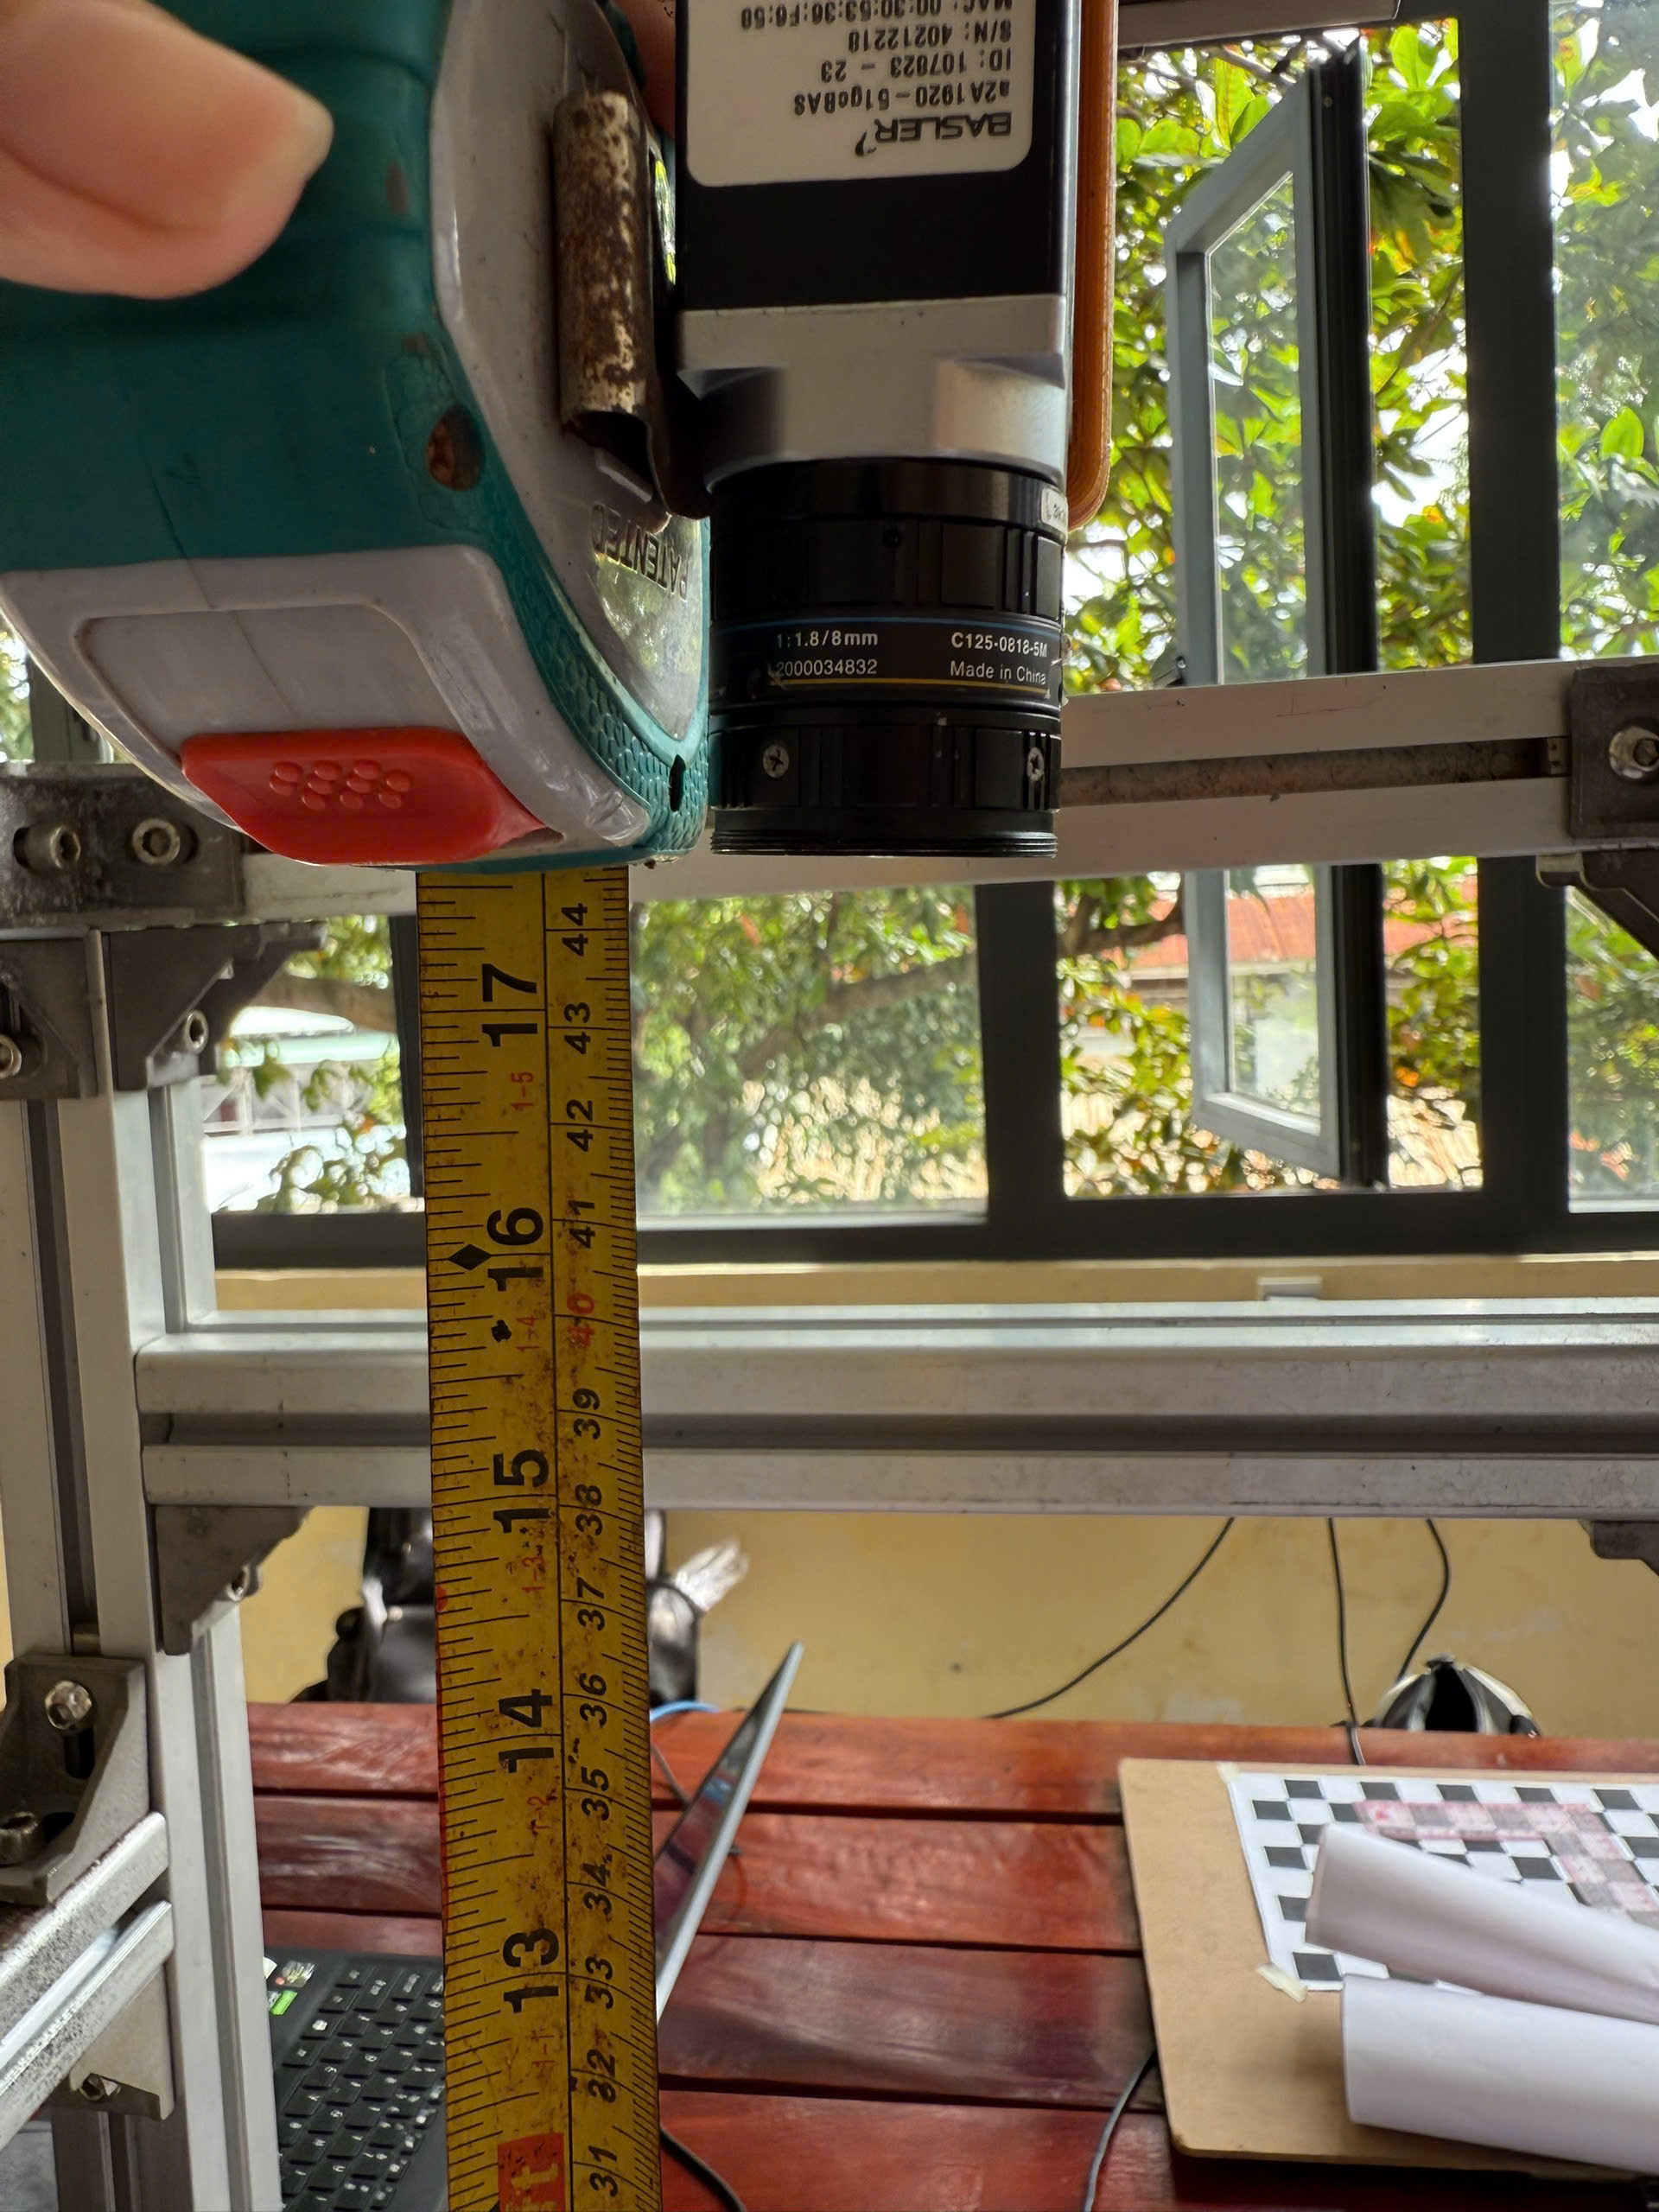
\includegraphics[width=1\textwidth]{pictures/section1/s1_p03.png}
                \caption{Working Distance thực tế}
                \label{fig:working_distance}
            \end{figure}
        \newpage
        \subsection{Tính toán theo lý thuyết}
            \subsubsection{Cơ sở lý thuyết}
                \begin{figure}[H]
                    \centering
                    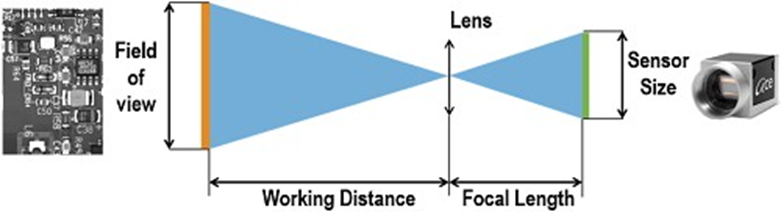
\includegraphics[width=1\textwidth]{pictures/section1/s1_p04.png}
                    \caption{Mô tả cách thức suy ra công thức tính toán}
                    \label{fig:working_distance}
                \end{figure}
            Theo tỷ lệ đồng dạng tam giác ở hình 4 ta có công thức như sau:
            \begin{equation}
                \frac{FOV}{Working\ Distance} = \frac{Sensor\ Size}{Focal\ Length}
            \end{equation}
            Suy ra:
            \begin{equation}
                FOV = \frac{Sensor\ Size \times Working\ Distance}{Focal\ Length}
            \end{equation}
            \subsubsection{Tính vùng quan sát, làm việc của camera với Working Distance đã chọn} 
                \hspace*{0.6cm}Với Working Distance = 445mm, Focal Length = 8mm, ta tính được:

                \textbf{FOV theo chiều ngang:}
                \begin{equation}
                    FOV_h = \frac{6.6 \times 445}{8} = 367.125mm
                \end{equation}

                \textbf{FOV theo chiều dọc:}
                \begin{equation}
                    FOV_v = \frac{4.1 \times 445}{8} = 228.0625mm
                \end{equation}

            \begin{itemize}
                \item FOV tính toán được: 367.125mm x 228.0625mm
                \item FOV thực tế: 388 mm x 238 mm
            \end{itemize}
            \cleardoublepage
            \subsection{Tính sai số của đường chéo FOV}
            \begin{itemize}
                \item Đường chéo theo lý thuyết tính từ kích thước FOV ở trên:
                \begin{equation}
                    \sqrt{367.125^2 + 228.0625^2} = 432.196mm
                \end{equation}
                \item Đường chéo FOV đo được thực tế:
                \begin{equation}
                    \sqrt{388^2 + 238^2} = 455.179 mm
                \end{equation}
                \item Sai số đường chéo FOV:
                \begin{equation}
                    \frac{|455.179 - 432.196|}{455.179} \times 100\% = 5.05\%
                \end{equation}
            \end{itemize}

            \subsection{Kiểm tra lại bằng công cụ Len Selector của nhà sản xuất}
            Để kiểm tra lại kết quả tính toán, nhóm sử dụng công cụ Len Selector của nhà sản xuất Basler để mô phỏng lại các thông số đã chọn. Kết quả thu được như hình bên dưới:
            \begin{figure}[H]
                \centering
                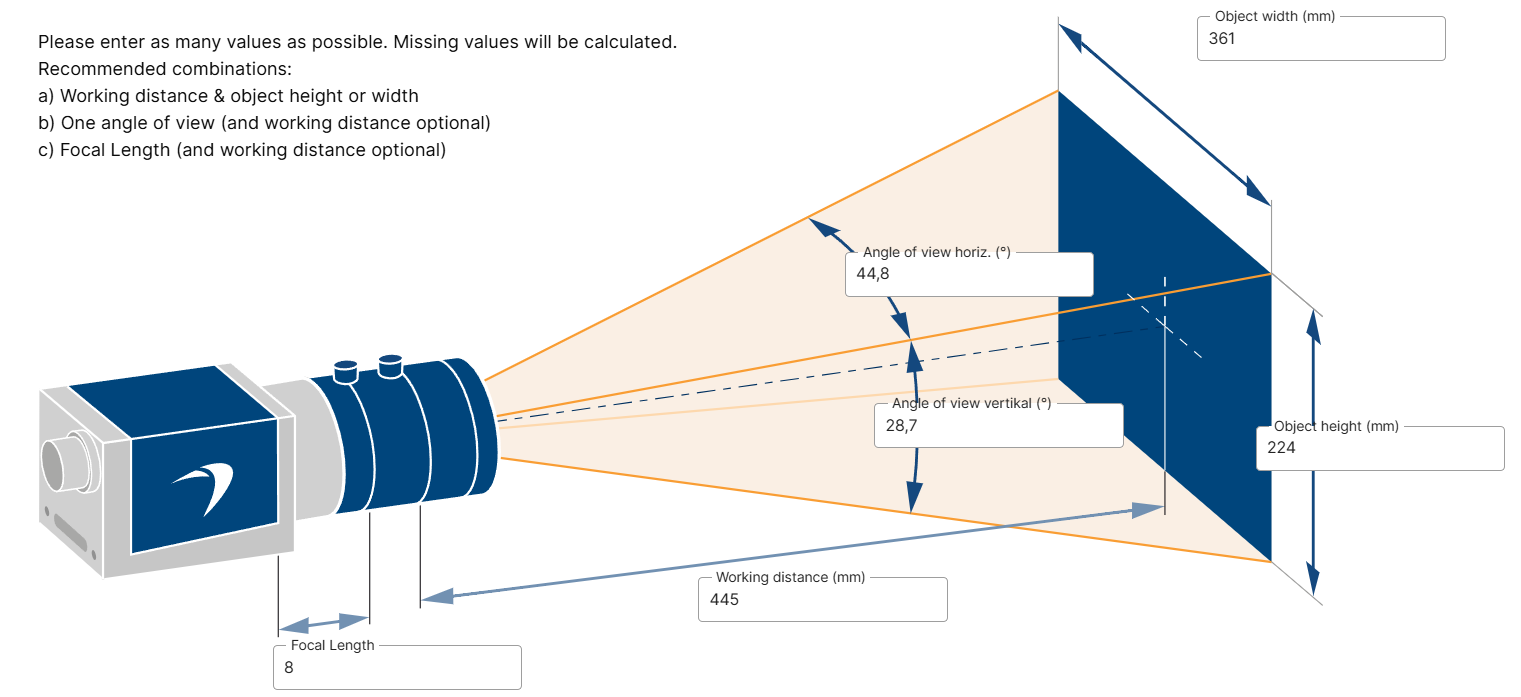
\includegraphics[width=1\textwidth]{pictures/section1/s1_p05.png}
                \caption{Đối chiếu các thông số bằng công cụ Len Selector của Basler}
                \label{fig:len_selector}
            \end{figure}
            Như vậy, các kết quả tính toán tương đối khớp với kết quả từ công cụ Len Selector của nhà sản xuất Basler.
            \cleardoublepage 